% ============================================================
%  Behavioral Clustering of NBA Prediction Markets on Kalshi
%  Math 364 — Machine Learning in Asset Pricing
%  Indigo Lee & William Walz · Claremont Graduate University
% ============================================================
\documentclass[10pt, aspectratio=169]{beamer}

\usetheme[progressbar=frametitle, block=fill]{metropolis}

\usepackage{booktabs}
\usepackage{graphicx}
\usepackage{amsmath}
\usepackage{xcolor}
\usepackage{tikz}
\usepackage{pgfplots}
\pgfplotsset{compat=1.18}

% ── Color palette ───────────────────────────────────────────
\definecolor{kalshi}{RGB}{26, 95, 180}    % deep blue
\definecolor{clusterA}{RGB}{31, 119, 180}
\definecolor{clusterB}{RGB}{255, 127, 14}
\definecolor{clusterC}{RGB}{44, 160, 44}
\definecolor{clusterD}{RGB}{214, 39, 40}
\definecolor{positive}{RGB}{44, 160, 44}
\definecolor{negative}{RGB}{214, 39, 40}

\setbeamercolor{frametitle}{bg=kalshi}
\setbeamercolor{progress bar}{fg=kalshi!70}
\setbeamercolor{alerted text}{fg=kalshi}

% ── Metadata ────────────────────────────────────────────────
\title{Behavioral Clustering of NBA\\Prediction Markets on Kalshi}
\subtitle{Math 364 — Machine Learning in Asset Pricing}
\author{Indigo Lee \and William Walz}
\institute{Claremont Graduate University}
\date{May 2026}

% ============================================================
\begin{document}
% ============================================================

% ── 1. TITLE SLIDE ──────────────────────────────────────────
\maketitle

% ── 2. WHAT IS KALSHI? ──────────────────────────────────────
\begin{frame}{What is Kalshi?}
  \begin{columns}[T]
    \begin{column}{0.55\textwidth}
      \textbf{A federally regulated prediction market exchange}

      \medskip
      Kalshi is the first CFTC-regulated exchange where retail investors
      can trade \alert{binary outcome contracts} on real-world events.

      \medskip
      \begin{block}{How contracts work}
        \begin{itemize}
          \item Each contract is a YES/NO question on a future event
          \item Resolves to \$1.00 if the stated condition is met (YES)
          \item Resolves to \$0.00 if not (NO)
          \item Market price at any moment $\approx$ crowd's
                \textbf{implied probability} of YES
        \end{itemize}
      \end{block}

      \medskip
      \begin{block}{Sports markets}
        NBA markets cover game winners, point totals, spreads,
        player statistics, and series outcomes --- generating
        continuous price histories spanning hours to weeks.
      \end{block}
    \end{column}
    \begin{column}{0.42\textwidth}
      \begin{block}{Example contract}
        \textit{``Will the Boston Celtics win Game 4?''}

        \smallskip
        \begin{tabular}{@{}ll@{}}
          \toprule
          Price & Interpretation \\
          \midrule
          \$0.30 & 30\% implied prob. of YES \\
          \$0.70 & 70\% implied prob. of YES \\
          \$0.99 & Near-certain YES \\
          \$0.01 & Near-certain NO \\
          \bottomrule
        \end{tabular}

        \medskip
        As news arrives (injury reports, tip-off, live score),
        the price updates continuously, tracing a
        \textbf{probability path} from open to resolution.
      \end{block}
    \end{column}
  \end{columns}
\end{frame}

% ── 3. RESEARCH QUESTION ────────────────────────────────────
\begin{frame}{Research Questions}
  \begin{alertblock}{Primary question}
    Do NBA prediction markets on Kalshi cluster into
    \textbf{distinct behavioral types} based on
    pre-resolution price dynamics?
  \end{alertblock}

  \bigskip
  \begin{block}{Secondary questions}
    \begin{enumerate}
      \item[\textbf{Q2}] Do those clusters \textbf{align with}
            Kalshi's stated market structure (game winner, player prop,
            total points, etc.), or do they \textbf{cut across} it?

            \smallskip
            \textit{Does the behavioral taxonomy match the contractual taxonomy?}

      \smallskip
      \item[\textbf{Q3}] Are some clusters \textbf{systematically
            mispriced} relative to actual resolution outcomes?

            \smallskip
            \textit{Does the crowd consistently over- or under-estimate
            the probability of YES for certain behavioral types?}
    \end{enumerate}
  \end{block}

  \bigskip
  \begin{center}
    \small
    \textit{Core insight: if price \emph{path shape} drives cluster membership,
    then behavioral dynamics reveal market structure that category labels alone cannot.}
  \end{center}
\end{frame}

% ── 4. DATA ─────────────────────────────────────────────────
\begin{frame}{Data}
  \begin{columns}[T]
    \begin{column}{0.48\textwidth}
      \begin{block}{Collection}
        \begin{itemize}
          \item \textbf{Source:} Kalshi REST API v2 (public)
          \item \textbf{Period:} February -- May 2026
          \item \textbf{Markets pulled:} 19{,}406 resolved NBA contracts
                across 24 series
          \item \textbf{After filtering} (duration $\geq$24 h,
                $\geq$10 candles): \textbf{946 markets}
          \item \textbf{Price history:} hourly OHLCV candlesticks
                per market (49{,}015 records total)
        \end{itemize}
      \end{block}

      \medskip
      \begin{block}{Market types in final sample}
        \footnotesize
        \begin{tabular}{@{}lr@{}}
          \toprule
          Type & $n$ \\
          \midrule
          Half spread   & 124 \\
          Player points & 117 \\
          Player prop   & 115 \\
          Game winner   & 113 \\
          Team total    & 110 \\
          Half total    & 108 \\
          Half winner   & 107 \\
          Total points  & 100 \\
          Other         &  52 \\
          \bottomrule
          \textbf{Total} & \textbf{946} \\
        \end{tabular}
      \end{block}
    \end{column}

    \begin{column}{0.50\textwidth}
      \begin{block}{Engineered features (per market)}
        \footnotesize
        \begin{tabular}{@{}ll@{}}
          \toprule
          Feature & Description \\
          \midrule
          \texttt{final\_prob} & YES prob.\ in final hour \\
          \texttt{change\_3h} & Price move, last 3 h \\
          \texttt{change\_24h} & Price move, last 24 h \\
          \texttt{total\_range} & Max$-$min over lifetime \\
          \texttt{volatility} & Std.\ dev.\ of hourly $\Delta p$ \\
          \texttt{drift\_slope} & OLS slope, final 24 h \\
          \texttt{days\_open} & Market lifetime (days) \\
          \texttt{time\_near\_50} & Fraction of life near 50\% \\
          \bottomrule
        \end{tabular}

        \medskip
        Features capture the \emph{shape} of each market's
        probability path, not its outcome level.
        All 8 features are z-scored before clustering.
      \end{block}
    \end{column}
  \end{columns}
\end{frame}

% ── 5. METHODOLOGY ──────────────────────────────────────────
\begin{frame}{Methodology}
  \begin{columns}[T]
    \begin{column}{0.48\textwidth}
      \begin{block}{K-means clustering}
        \begin{enumerate}
          \item Represent each market as an 8-dimensional
                feature vector (z-scored)
          \item K-means partitions markets into $k$ groups by
                minimizing within-cluster variance
          \item Cluster $\approx$ ``markets with similar
                price path behavior''
          \item 10 random restarts; best solution kept
        \end{enumerate}
      \end{block}

      \medskip
      \begin{block}{Choosing $k$}
        \begin{itemize}
          \item \textbf{Elbow method:} plot inertia
                (within-cluster SSE) vs.\ $k$; look for
                the bend where gains diminish
          \item \textbf{Silhouette score:} measures
                how well-separated clusters are;
                higher = better
          \item We enforce $k \geq 4$ to ensure
                behaviorally distinct types beyond
                the trivial YES/NO split
        \end{itemize}
      \end{block}
    \end{column}

    \begin{column}{0.50\textwidth}
      \begin{block}{What features capture behaviorally}
        \footnotesize
        \begin{tabular}{@{}p{2.6cm}p{3.5cm}@{}}
          \toprule
          Feature & Behavioral meaning \\
          \midrule
          \texttt{final\_prob} & Was the market priced as
                                  a favorite or underdog? \\[3pt]
          \texttt{change\_24h} & Did the crowd update strongly
                                  in the final day? \\[3pt]
          \texttt{total\_range} & How uncertain was the outcome
                                   at any point? \\[3pt]
          \texttt{volatility} & How rough was the price path? \\[3pt]
          \texttt{time\_near\_50} & How long did the market sit
                                    in genuine uncertainty? \\[3pt]
          \texttt{days\_open} & Was this a long-horizon or
                                 short-horizon market? \\
          \bottomrule
        \end{tabular}
      \end{block}

      \medskip
      \begin{block}{Calibration test}
        For each cluster: two-sided binomial test.
        $H_0$: final market price is an unbiased predictor
        of YES resolution rate.
      \end{block}
    \end{column}
  \end{columns}
\end{frame}

% ── 6. ELBOW CURVE ──────────────────────────────────────────
\begin{frame}{Selecting the Number of Clusters}
  \begin{columns}[T]
    \begin{column}{0.58\textwidth}
      \begin{figure}
        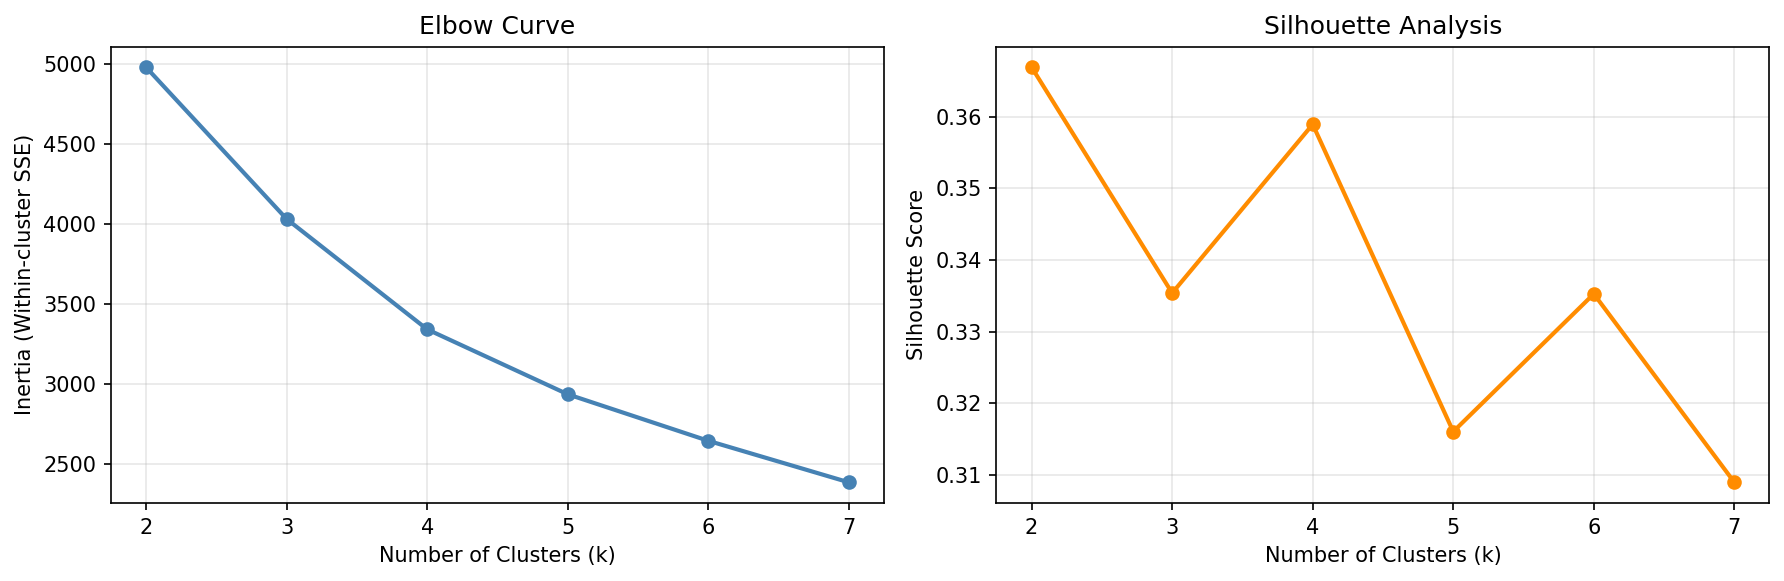
\includegraphics[width=\textwidth]{elbow_curve.png}
        \caption{Inertia (left) and silhouette score (right) for $k = 2\text{--}7$.}
      \end{figure}
    \end{column}
    \begin{column}{0.40\textwidth}
      \begin{block}{Reading the charts}
        \begin{itemize}
          \item The elbow in inertia occurs at $k = 3$--$4$,
                after which gains diminish
          \item Silhouette peaks globally at $k = 2$
                (trivially separates YES-side from NO-side markets)
          \item Among $k \geq 4$, \textbf{$k = 4$} achieves the
                highest silhouette score of \textbf{0.36}
        \end{itemize}
      \end{block}

      \medskip
      \begin{alertblock}{Selected: $k = 4$}
        Four clusters yield meaningful behavioral distinctions
        while maintaining good cluster cohesion.
        The silhouette score of 0.36 confirms the partition
        is well above chance.
      \end{alertblock}
    \end{column}
  \end{columns}
\end{frame}

% ── 7. CLUSTER SCATTER ──────────────────────────────────────
\begin{frame}{Cluster Scatter Plot (PCA)}
  \begin{columns}[T]
    \begin{column}{0.58\textwidth}
      \begin{figure}
        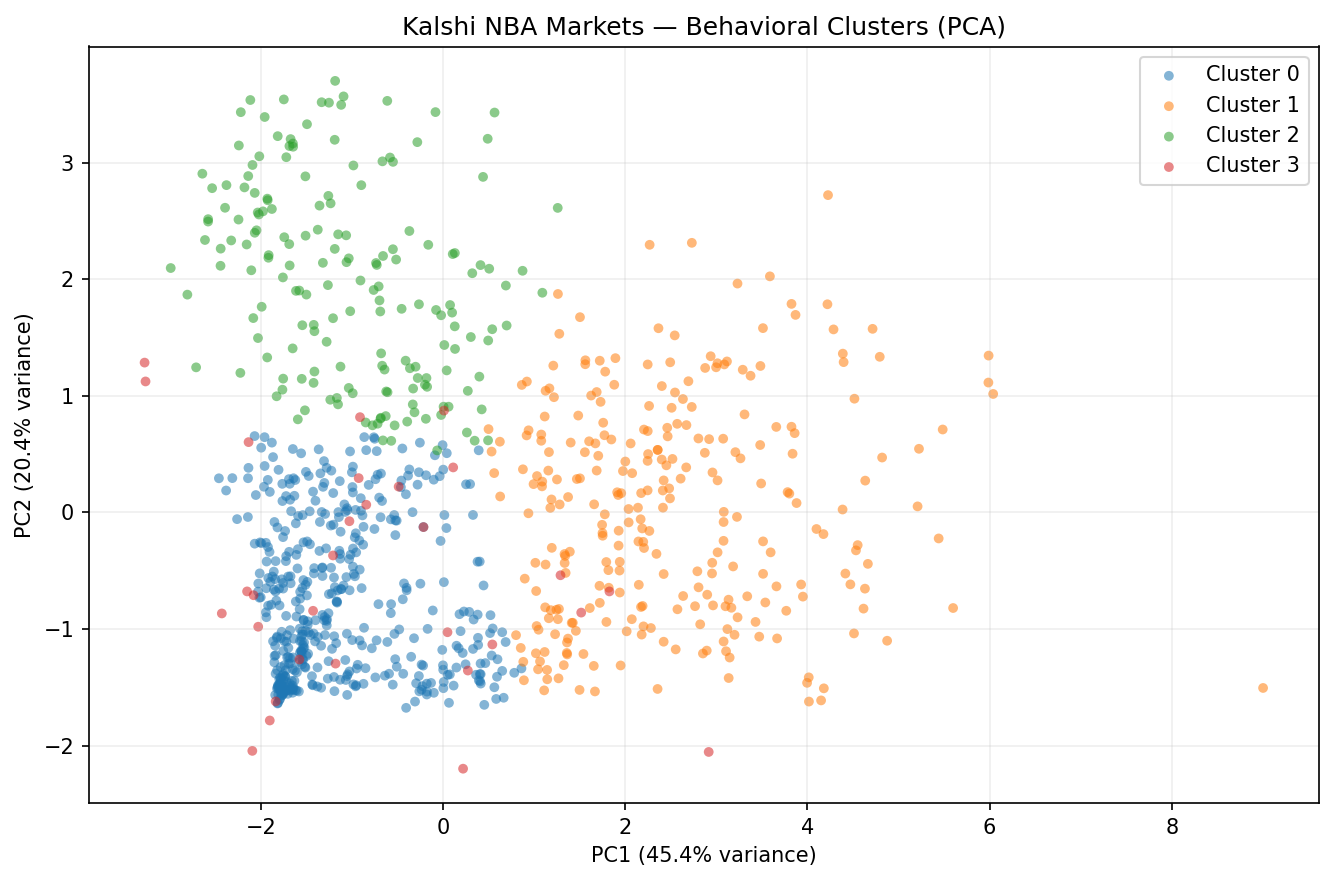
\includegraphics[width=\textwidth]{cluster_scatter.png}
        \caption{All 946 markets projected onto the first two PCA
          components, colored by cluster assignment.}
      \end{figure}
    \end{column}
    \begin{column}{0.40\textwidth}
      \begin{block}{Interpreting the scatter}
        Each point is one resolved NBA market.
        Axes are the first two principal components of the
        8-dimensional feature space, capturing the dominant
        directions of behavioral variation.

        \medskip
        \begin{itemize}
          \item \textbf{PC1} (horizontal) primarily
                separates markets by \texttt{final\_prob}
                --- how the market resolved
          \item \textbf{PC2} (vertical) captures
                path dynamics: range, volatility,
                time near 50\%
        \end{itemize}
      \end{block}

      \medskip
      \begin{block}{Cluster separation}
        Clusters 0 and 1 are tightly packed and well-separated
        (consistent price behavior). Clusters 2 and 3
        occupy more diffuse regions, reflecting higher
        within-cluster variation in path shape.
      \end{block}
    \end{column}
  \end{columns}
\end{frame}

% ── 8. FEATURE HEATMAP ──────────────────────────────────────
\begin{frame}{Cluster Profiles: What Each Cluster Behaves Like}
  \begin{columns}[T]
    \begin{column}{0.52\textwidth}
      \begin{figure}
        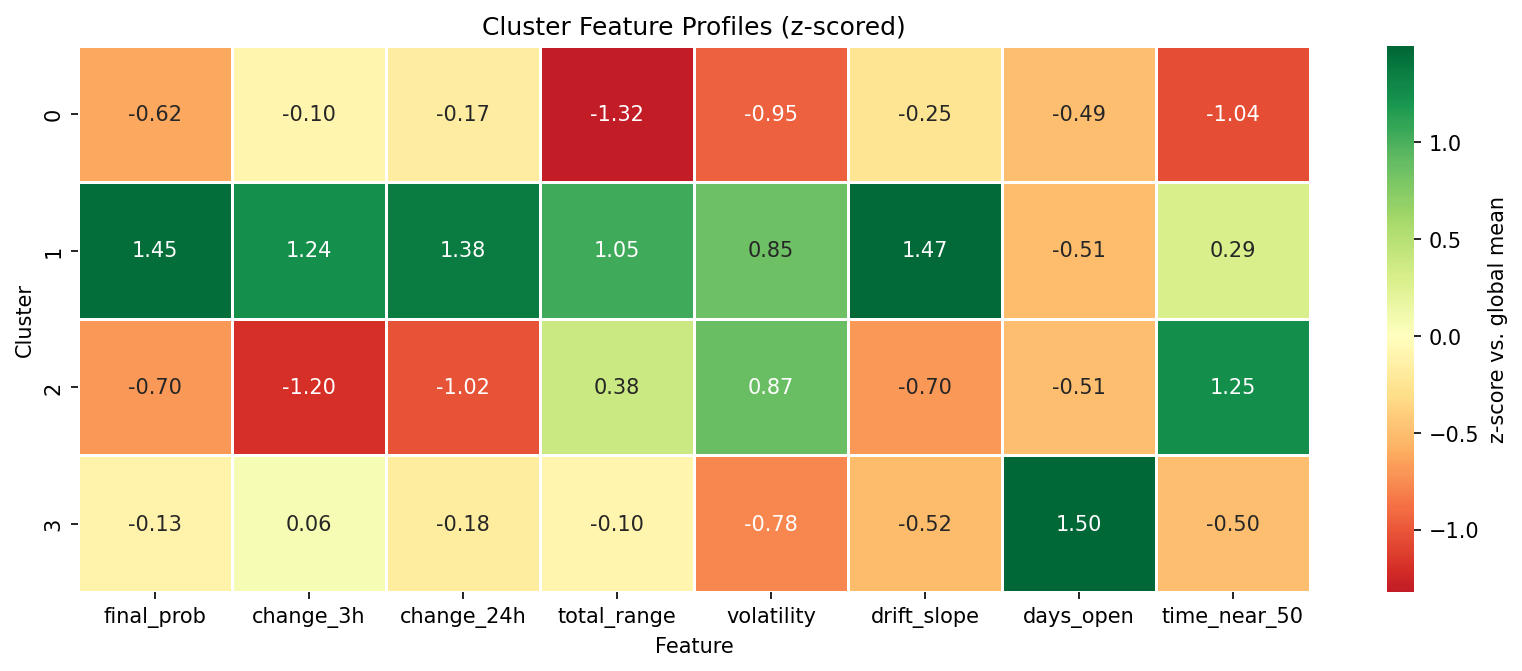
\includegraphics[width=\textwidth]{feature_heatmap.png}
        \caption{Mean feature value per cluster (z-scored across clusters).
          Red = above average; green = below average.}
      \end{figure}
    \end{column}
    \begin{column}{0.46\textwidth}
      \footnotesize
      \begin{block}{\textcolor{clusterA}{Cluster 0 — ``Stable Underdogs''} ($n=453$)}
        Consistently priced $<$25\%, almost never near 50\%,
        low volatility. Outcome was obvious from market open.
        Resolved NO 86\% of the time.
      \end{block}

      \smallskip
      \begin{block}{\textcolor{clusterB}{Cluster 1 — ``Late Movers''} ($n=286$)}
        Started near 50/50, then surged +48 cents in the
        final 24 hours. Wide range (0.73). Resolved YES 84\%
        of the time --- the crowd moved decisively and correctly.
      \end{block}

      \smallskip
      \begin{block}{\textcolor{clusterC}{Cluster 2 — ``Volatile Near-Misses''} ($n=177$)}
        Spent 46\% of lifetime near 50\%, then collapsed
        toward NO. Wide range (0.59), strong negative drift.
        Markets that \emph{looked} contested but resolved NO.
      \end{block}

      \smallskip
      \begin{block}{\textcolor{clusterD}{Cluster 3 — ``Long-Horizon Markets''} ($n=30$)}
        Open for $\sim$14 days on average. Series-outcome
        contracts. Low short-term volatility; moderate
        uncertainty throughout; resolved YES only 27\%.
      \end{block}
    \end{column}
  \end{columns}
\end{frame}

% ── 9. MARKET TYPE BREAKDOWN ────────────────────────────────
\begin{frame}{Do Clusters Align with Market Type?}
  \begin{columns}[T]
    \begin{column}{0.54\textwidth}
      \begin{figure}
        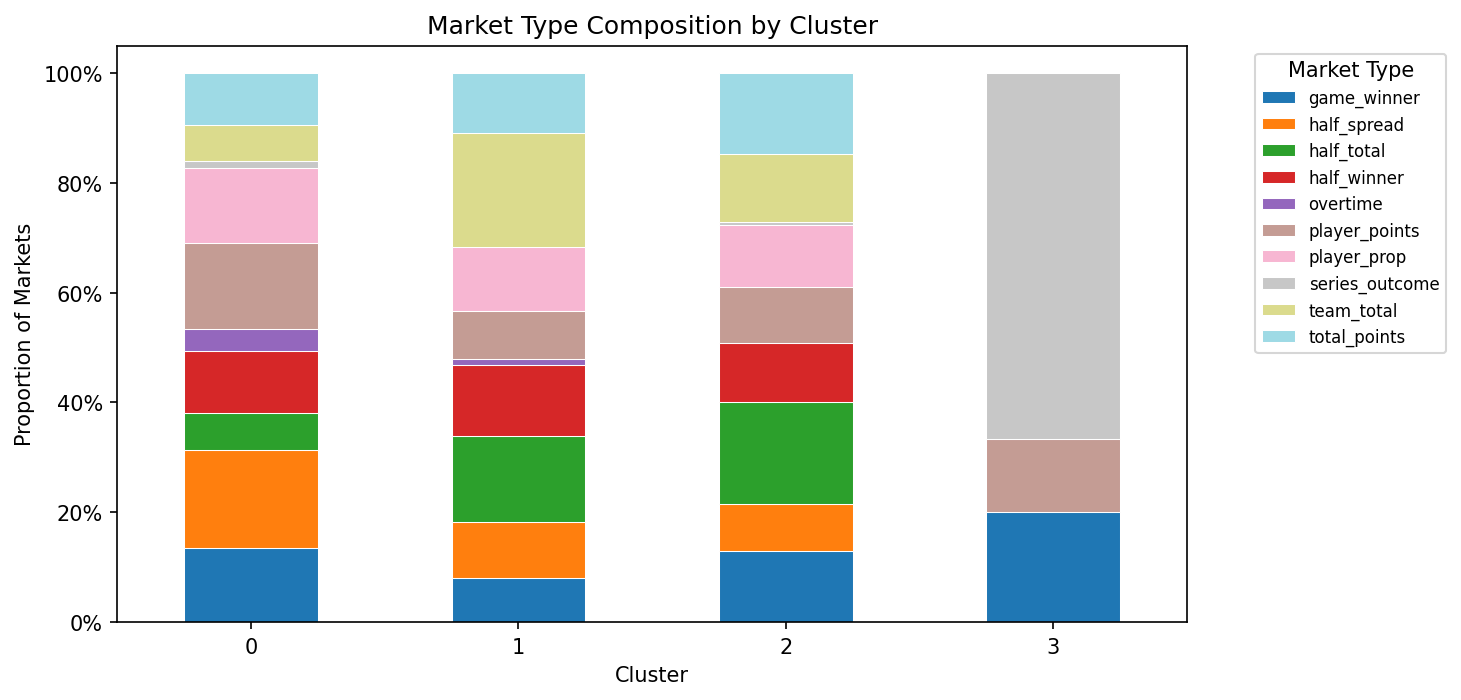
\includegraphics[width=\textwidth]{sport_breakdown.png}
        \caption{Market type composition within each cluster (row-normalized to 100\%).}
      \end{figure}
    \end{column}
    \begin{column}{0.44\textwidth}
      \begin{alertblock}{Key finding: clusters cut \emph{across} market type}
        Every cluster contains both game-outcome markets
        and player prop markets. The behavioral taxonomy
        does \textbf{not} mirror Kalshi's stated categories.
      \end{alertblock}

      \medskip
      \begin{block}{What this means}
        \begin{itemize}
          \item A game winner market and a player prop market
                can share the same price-path behavior ---
                they end up in the same cluster
          \item The relevant dimension is
                \textbf{how the crowd updates beliefs},
                not what the contract is \emph{about}
          \item Information flow in NBA prediction markets
                is structurally similar across contract types:
                same dynamics, different underlying events
        \end{itemize}
      \end{block}

      \medskip
      \begin{block}{Exception: Cluster 3}
        Series-outcome markets ($\sim$67\% of Cluster 3) are
        the one category that forms its own behavioral niche
        --- driven by their much longer duration, not their
        subject matter.
      \end{block}
    \end{column}
  \end{columns}
\end{frame}

% ── 10. MISPRICING ──────────────────────────────────────────
\begin{frame}{Mispricing Analysis}
  \begin{columns}[T]
    \begin{column}{0.50\textwidth}
      \begin{figure}
        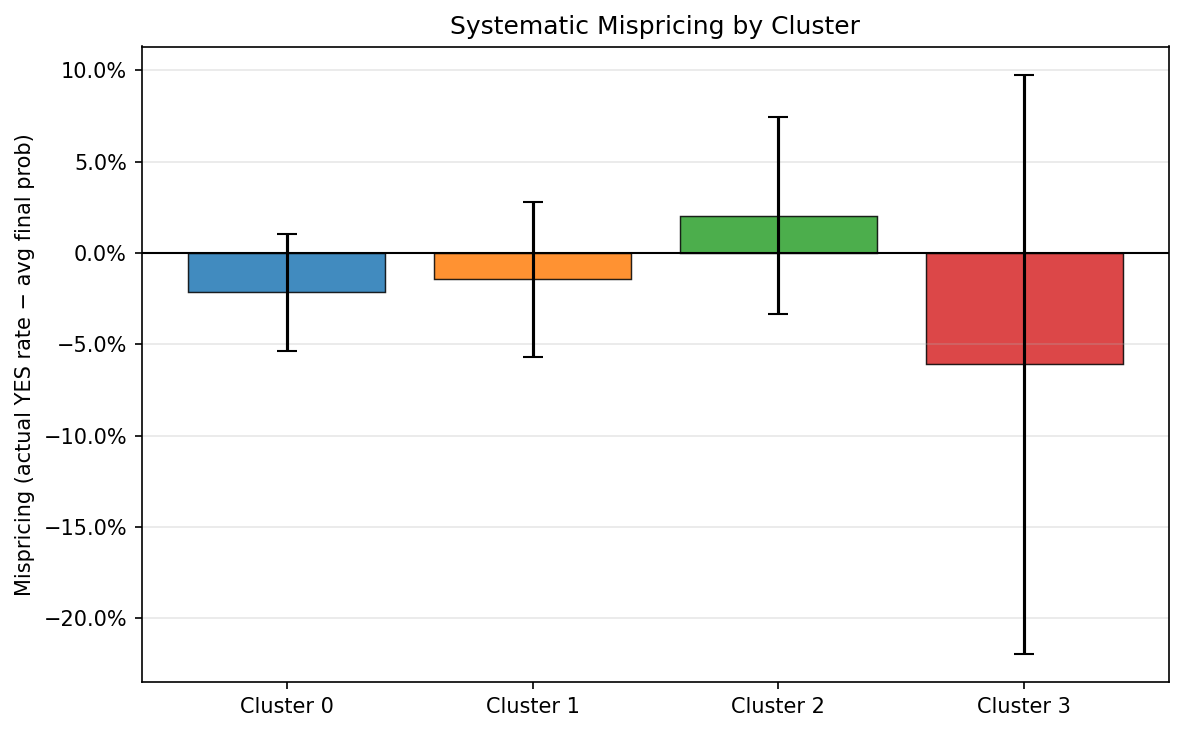
\includegraphics[width=\textwidth]{mispricing_chart.png}
        \caption{Mispricing per cluster (actual YES rate $-$ avg.\ final prob.)
          with 95\% Wald CIs. No asterisk = not significant at $\alpha=0.05$.}
      \end{figure}
    \end{column}
    \begin{column}{0.48\textwidth}
      \begin{block}{Results}
        \footnotesize
        \begin{tabular}{@{}crrrl@{}}
          \toprule
          Cluster & $n$ & Avg.\ prob & YES rate & Mispricing \\
          \midrule
          0 & 453 & 16.3\% & 14.1\% & $-2.1$ pp \\
          1 & 286 & 85.4\% & 83.9\% & $-1.5$ pp \\
          2 & 177 & 13.8\% & 15.8\% & $+2.1$ pp \\
          3 &  30 & 32.8\% & 26.7\% & $-6.1$ pp \\
          \bottomrule
        \end{tabular}
        \vspace{2pt}

        All $p$-values $> 0.22$; no cluster is significantly
        mispriced at $\alpha = 0.05$.
      \end{block}

      \medskip
      \begin{block}{Interpretation}
        \begin{itemize}
          \item \textbf{Clusters 0 \& 1} (stable underdogs \&
                late movers): slightly over-priced relative
                to outcomes --- markets slightly overestimate YES
          \item \textbf{Cluster 2} (volatile near-misses):
                slightly under-priced --- the crowd underestimates
                how often these ``contested'' markets resolve YES
          \item \textbf{Cluster 3} (long-horizon): largest gap
                ($-6.1$ pp) but only 30 markets; low statistical power
          \item \textbf{Overall:} Kalshi NBA markets appear
                \textbf{well-calibrated} --- no exploitable edge found
        \end{itemize}
      \end{block}
    \end{column}
  \end{columns}
\end{frame}

% ── 11. CALIBRATION CURVES ──────────────────────────────────
\begin{frame}{Calibration Curves}
  \begin{columns}[T]
    \begin{column}{0.54\textwidth}
      \begin{figure}
        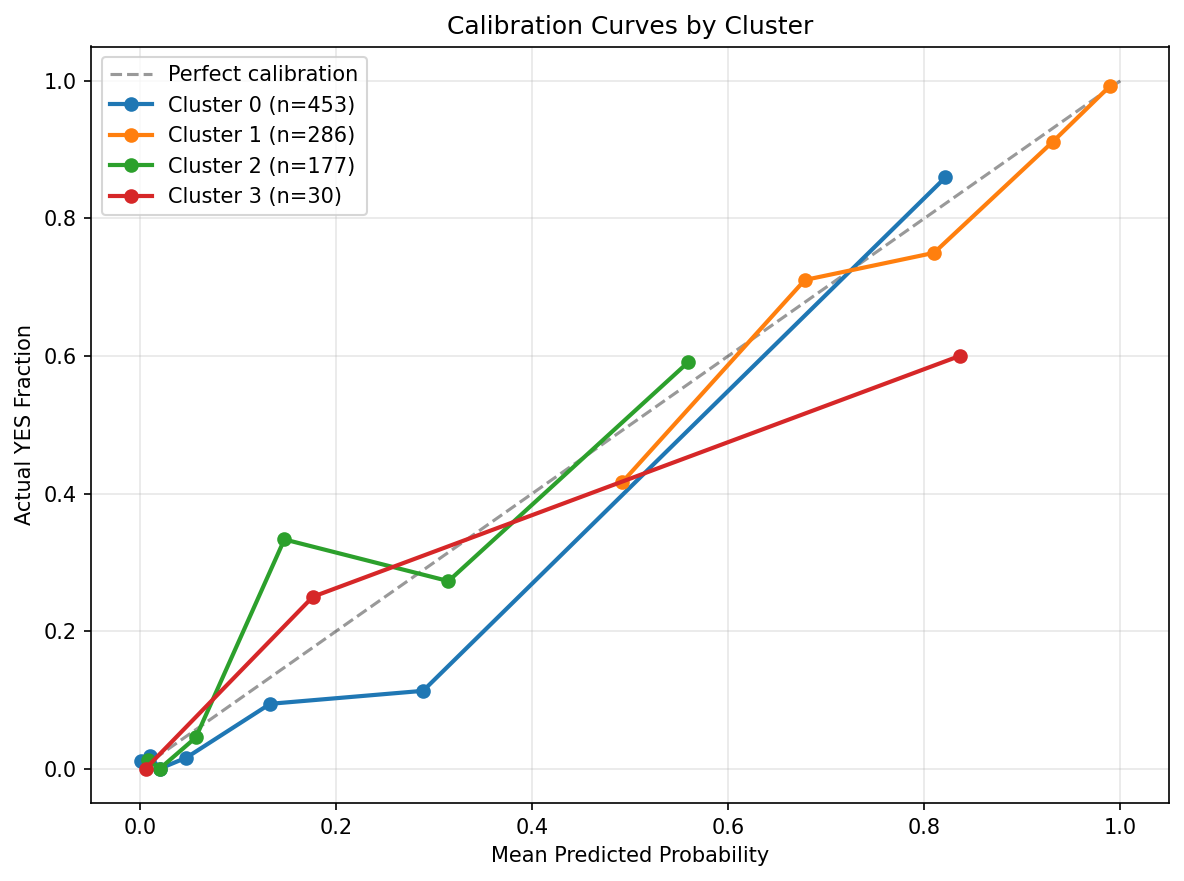
\includegraphics[width=\textwidth]{calibration_curve.png}
        \caption{Quantile-binned calibration curves per cluster.
          A market that lies on the dashed diagonal is
          perfectly calibrated.}
      \end{figure}
    \end{column}
    \begin{column}{0.44\textwidth}
      \begin{block}{What calibration means}
        A market is \textbf{well-calibrated} if, among all
        contracts priced at $p$, a fraction $p$ actually
        resolve YES. Perfect calibration = the diagonal.

        \medskip
        Good calibration is a necessary (but not sufficient)
        condition for market efficiency.
      \end{block}

      \medskip
      \begin{block}{Findings by cluster}
        \begin{itemize}
          \item \textbf{Clusters 0 \& 1} hug the diagonal
                closely at their respective ends of the
                probability range --- these markets are
                highly calibrated
          \item \textbf{Cluster 2} shows slight deviation
                near the 50\% range: the market slightly
                underestimates YES probability for
                ``contested'' markets
          \item \textbf{Cluster 3} has too few observations
                to draw firm calibration conclusions
          \item \textbf{Takeaway:} NBA prediction markets
                efficiently aggregate information and
                produce reliable probability estimates
        \end{itemize}
      \end{block}
    \end{column}
  \end{columns}
\end{frame}

% ── 12. CONCLUSIONS ─────────────────────────────────────────
\begin{frame}{Conclusions}
  \begin{columns}[T]
    \begin{column}{0.48\textwidth}
      \begin{alertblock}{Q1: Do distinct behavioral types exist?}
        \textbf{Yes.} K-means finds 4 well-separated clusters
        (silhouette = 0.36) in the 8-dimensional feature space.
        The four types are: Stable Underdogs, Late Movers,
        Volatile Near-Misses, and Long-Horizon Markets.
      \end{alertblock}

      \medskip
      \begin{alertblock}{Q2: Align with or cut across Kalshi's structure?}
        \textbf{Cut across.} Every cluster mixes game-winner
        markets with player prop markets. Behavioral
        dynamics --- not contract category --- are the true
        organizing principle. The exception is Cluster 3,
        where duration alone drives separation.
      \end{alertblock}

      \medskip
      \begin{alertblock}{Q3: Systematic mispricing?}
        \textbf{Not significantly.} No cluster shows
        statistically significant calibration failure
        at $\alpha=0.05$. Kalshi NBA markets are
        well-calibrated overall.
      \end{alertblock}
    \end{column}
    \begin{column}{0.50\textwidth}
      \begin{block}{What the clusters reveal}
        The primary axes of NBA prediction market behavior are:
        \begin{enumerate}
          \item \textbf{Where a market resolves:} near 0 (underdog)
                or near 1 (favorite) --- the dominant dimension
          \item \textbf{How it gets there:} steadily priced from
                open (Cluster 0) vs.\ sharp late convergence
                (Cluster 1) vs.\ contested-then-collapsed
                (Cluster 2)
          \item \textbf{How long it was open:} short-term
                game-day contracts vs.\ multi-week
                series markets (Cluster 3)
        \end{enumerate}
      \end{block}

      \medskip
      \begin{block}{Trading implications}
        No cluster shows a \emph{significant} exploitable
        edge after multiple comparison adjustment.
        The mild under-pricing in Cluster 2 (volatile
        near-misses, $+2.1$ pp) is the closest candidate,
        but with $n=177$ and $p=0.44$ it does not clear
        the significance bar at this sample size.
        Larger datasets and live testing would be needed.
      \end{block}
    \end{column}
  \end{columns}
\end{frame}

% ── 13. REFERENCES ──────────────────────────────────────────
\begin{frame}[allowframebreaks]{References}
  \footnotesize
  \begin{thebibliography}{9}

    \bibitem{kalshi_api}
    Kalshi Inc.
    \textit{Kalshi Trading API v2 Documentation.}
    \url{https://api.elections.kalshi.com/trade-api/v2}, 2026.

    \bibitem{wolfers_prediction}
    J.\ Wolfers and E.\ Zitzewitz.
    ``Prediction markets.''
    \textit{Journal of Economic Perspectives}, 18(2):107--126, 2004.

    \bibitem{arrow_pm}
    K.\ Arrow, R.\ Forsythe, M.\ Gorham, et al.
    ``The promise of prediction markets.''
    \textit{Science}, 320(5878):877--878, 2008.

    \bibitem{manski}
    C.\ Manski.
    ``Interpreting the predictions of prediction markets.''
    \textit{Economics Letters}, 91(3):425--429, 2006.

    \bibitem{kmeans}
    J.\ MacQueen.
    ``Some methods for classification and analysis of
    multivariate observations.''
    \textit{Proceedings of the 5th Berkeley Symposium on
    Mathematical Statistics and Probability}, 1:281--297, 1967.

    \bibitem{silhouette}
    P.\ J.\ Rousseeuw.
    ``Silhouettes: a graphical aid to the interpretation
    and validation of cluster analysis.''
    \textit{Journal of Computational and Applied Mathematics},
    20:53--65, 1987.

    \bibitem{sklearn}
    F.\ Pedregosa et al.
    ``Scikit-learn: Machine learning in Python.''
    \textit{Journal of Machine Learning Research},
    12:2825--2830, 2011.

    \bibitem{snowberg}
    E.\ Snowberg and J.\ Wolfers.
    ``Explaining the favorite-longshot bias: Is it risk-love
    or misperceptions?''
    \textit{Journal of Political Economy}, 118(4):723--746, 2010.

    \bibitem{tetlock}
    P.\ E.\ Tetlock.
    \textit{Expert Political Judgment: How Good Is It?
    How Can We Know?}
    Princeton University Press, 2005.

  \end{thebibliography}
\end{frame}

% ============================================================
\end{document}
